\documentclass[11pt]{article}
\usepackage{fancyhdr} 
\pagestyle{fancy}
\fancyhf{}
\fancyheadoffset{0cm}
\renewcommand{\headrulewidth}{0pt} 
\renewcommand{\footrulewidth}{0pt}
\fancyhead[R]{{\color{gray!50}Page Number: \thepage { \small (out of 7 pages)}}}
\fancypagestyle{plain}{%
  \fancyhf{}%
  \fancyhead[R]{\thepage}%
}




\usepackage{graphicx}
\usepackage[margin=.5in]{geometry} 
\usepackage{amsmath,amsthm,amssymb}
%\usepackage{gensymb}
  \usepackage{hyperref}
  \usepackage{pdfpages} 
  %\usepackage[table]{xcolor}
  
 %\usepackage{xcolor} % Required for specifying colors by name
\definecolor{ocre}{RGB}{52,177,201} % Define the orange color used for highlighting throughout the book

% Font Settings
\usepackage{avant} % Use the Avantgarde font for headings
%\usepackage{times} % Use the Times font for headings
\usepackage{mathptmx} % Use the Adobe Times Roman as the default text font together with math symbols from the Sym­bol, Chancery and Com­puter Modern fonts

%\usepackage{microtype} % Slightly tweak font spacing for aesthetics
%\usepackage[utf8]{inputenc} % Required for including letters with accents
\usepackage[T1]{fontenc} % Use 8-bit encoding that has 256 glyphs
%\usepackage{soul}
\usepackage{undertilde}
%\usepackage{accents}
\newcommand{\StandardLM}{\by=\bX \bbeta +{\epsilonbf}}

\usepackage{xcolor}
\usepackage{xparse}
\definecolor{lightGray}{gray}{0.95}
\definecolor{lightGrayOne}{gray}{0.9}
\definecolor{lightBlueOne}{RGB}{204, 255, 255}
\definecolor{lightBlueTwo}{RGB}{204, 238, 255}
\definecolor{lightBlueThree}{RGB}{204, 204, 255}
\definecolor{AltBlue}{RGB}{119,14,161}
\definecolor{Orchid}{RGB}{186,85,211}

\definecolor{BGBlue}{RGB}{220,221,252}
\definecolor{BGBlueOne}{RGB}{204,229,255}

\definecolor{DarkGreenOne}{RGB}{34,139,34}

\definecolor{BGGreen}{RGB}{240,243,245}
\definecolor{lightGreenOne}{RGB}{179, 255, 179}
\definecolor{lightGreenTwo}{RGB}{198, 255, 179}
\definecolor{lightGreenThree}{RGB}{243, 255, 230}
\definecolor{AltGreen}{RGB}{193, 240, 240}

\definecolor{BOGreen}{RGB}{180,0,0}
\definecolor{BGGreenOne}{RGB}{220,250,220}

\definecolor{lightBrownOne}{RGB}{255, 221, 204}
\definecolor{lightBrownTwo}{RGB}{255, 229, 204}
\definecolor{lightBrownThree}{RGB}{242, 217, 230}


\definecolor{HLTGreen}{RGB}{230,244,215}
\definecolor{ExcBrown}{RGB}{153,0,0}
\definecolor{ExcBGBrown}{RGB}{255,204,204}
\definecolor{BGYellowOne}{RGB}{255,235,208}
\definecolor{BGPink}{RGB}{255,215,240}

\newcommand{\MakeVec}[1]{{\utilde{\bf #1}}}

\NewDocumentCommand{\MCOption}{O{1.75in} m}{
\TextInBoxTwo[BGPink]{ #1 } {\TextInBoxTwo[white]{.1 in }{ \quad}\HLT{#2}}
}

 \NewDocumentCommand{\ThreeChoices}{O{Do not Know}O{Not confident}O{Confident}}{
\MCOption{#1} \MCOption{#2} \MCOption{#3}
}
 
\NewDocumentCommand{\OneBlock}{ O{HLTGreen} m m }{\colorbox{#1}{\begin{minipage}{#2} $ #3$ \end{minipage}}}

\NewDocumentCommand{\HLT}{ O{HLTGreen} m }{\colorbox{#1}{#2}}
%\NewDocumentCommand{\HLTEQ}{ O{HLTGreen} m }{\colorbox{#1}{$#2$}}
\NewDocumentCommand{\HLTEQ}{ O{white} m }{\colorbox{#1}{$#2$}}

%\newcommand{\HLT}[1]{\colorbox{HLTGreen}{#1}}
\newcommand{\DEHLT}[1]{\colorbox{lightGrayOne}{\color{white} #1}}

\newcommand{\TextInBoxOne}[2]{  {\fcolorbox{white}{lightGrayOne}{\begin{minipage}{#1}  #2 \end{minipage}}}}


\NewDocumentCommand{\TextInBoxTwo}{ O{lightGrayOne} m m } {{\fcolorbox{white}{#1}{\begin{minipage}{#2} { #3} \end{minipage}}}}


\newcommand{\TextInBox}[2]{  {\fcolorbox{BGGreen}{BGGreen}{\begin{minipage}{#1}  #2 \end{minipage}}}}
\newcommand{\TextInBoxCol}[2]{
\fcolorbox{BGBlue}{BGBlue}{%
\begin{minipage}{#1}
 {\color{AltBlue} #2}
\end{minipage}}%
}

\NewDocumentCommand{\TxtBnd}{ O{lightBrownOne} m m } {{\fcolorbox{white}{#1}{\begin{minipage}{#2} { #3} \end{minipage}}}}


\newcommand{\BandInTopBox}[2]{
\fcolorbox{AltBlue}{AltBlue}{%
\begin{minipage}{#1}{ {\color{white}  #2 \hspace{.1in}} }
\end{minipage}}%
}


\newcommand{\TextInBoxThm}[2]{
\fcolorbox{AltBlue}{lightGray}{%
\begin{minipage}{#1}
 {\color{black} #2}
\end{minipage}}%
}

\newcommand{\TextInBoxThmOne}[2]{
\fcolorbox{BGBlue}{BGBlueOne}{%
\begin{minipage}{#1}
 {\color{AltBlue} #2}
\end{minipage}}%
}

\newcommand{\TextInBoxLem}[2]{
\fcolorbox{BGBlue}{lightGray}{%
\begin{minipage}{#1}
 {\color{black} #2}
\end{minipage}}%
}



\newcommand{\TextInBoxLemOne}[2]{
\vspace{.02 in}
\noindent
\fcolorbox{BGBlue}{BGBlue}{%
\begin{minipage}{#1}
 {\color{AltBlue} #2}
\end{minipage}}%
}



\newcommand{\DefBox}[1]{
%\vspace{.1 in}
\noindent
\TextInBoxLem{4.5 in }{
\BandInTopBox{4.4 in }{}
\TextInBoxLemOne{4.4 in }{
#1
}}}





\newcommand{\DefBoxOne}[2]{
%\vspace{.1 in}
\noindent
\TextInBoxLem{4.5 in }{
\BandInTopBox{4.4 in }{#1}
\TextInBoxLemOne{4.4 in }{
#2
}}}


\newcommand{\ThmBox}[2]{
\noindent
\TextInBoxThm{4.4 in }{
\TextInBoxThmOne{4.4 in }{
#1}
#2}
}

\newcommand{\LemBox}[2]{
\noindent
\TextInBoxLem{4.5 in }{
\TextInBoxLemOne{4.4 in }{
#1}
#2}
}

\newcommand{\PropBox}[2]{
\vspace{.1 in}
\noindent
\TextInBoxLem{4.5 in }{
\TextInBoxLemOne{4.4 in }{
#1}
#2}
}




\newcommand{\TextInBoxExc}[2]{
\noindent
\fcolorbox{white}{BGGreenOne}{%
\begin{minipage}{#1}
 {\color{black} #2}
\end{minipage}}%
}


\newcommand{\TextInBoxExample}[2]{
\noindent
\fcolorbox{white}{BGPink}{%
\begin{minipage}{#1}
 {\color{black} #2}
\end{minipage}}%
}


\newcommand{\ExerciseBox}[1]{
\noindent
%\TextInBoxLem{6 in }{
\TextInBoxExc{6 in }{
#1}
%#2}
}


\newcommand{\ExampleBox}[1]{
\noindent
%\TextInBoxLem{6 in }{
\TextInBoxExample{6 in }{
#1}
%#2}
}

\NewDocumentCommand{\CommentBox}{ O{BGBlue}  m }{
\TextInBoxLem{5.5in }{
{\bf Comment:}\\
\TextInBoxLemOne{5.4 in }{
#2}}
}



\newcommand{\HLTY}[1]{\HLTEQ[yellow]{#1}}
\newcommand{\HLTW}[1]{\HLTEQ[white]{#1}}



\newcommand{\qBox}[1]{
  \begin{tikzpicture}
\node[draw=none,shade,
      top color=lightGrayOne,
      bottom color=lightGray,
      rounded corners=2pt,
      blur shadow={shadow blur steps=5}
    ] at (0,0) {    \noindent 
\fcolorbox{white}{BGBlue}{%
\begin{minipage}{4.55 in}
 {\color{black} {
 #1}}
\end{minipage}  }%
 };
 
    \end{tikzpicture}
}
 
 


 

\newcommand{\qBoxCol}[2]{
  \begin{tikzpicture}
\node[draw=none,shade,
      top color=lightGrayOne,
      bottom color=lightGray,
      rounded corners=2pt,
      blur shadow={shadow blur steps=5}
    ] at (0,0) {    \noindent
\fcolorbox{white}{#1}{%
%\begin{minipage}{4.55 in}
\begin{minipage}{4.55 in}
 {
 \color{black} {
 #2}}
\end{minipage}  }%
 };
 
    \end{tikzpicture}
}
  
  
  
  
  
  

\NewDocumentCommand{\qBrd}{O{4.55 in} m m}{
  \begin{tikzpicture}
\node[draw=none,shade,
      top color=#2,
      bottom color=#2,
      rounded corners=2pt,
      blur shadow={shadow blur steps=5}
    ] at (0,0) {    \begin{minipage}{#1}
 {
 \color{black} {
 #3}}
\end{minipage} 

 };
 
    \end{tikzpicture}
}
    
  
  
  
  
\NewDocumentCommand{\qbx}{O{4.55 in} m m}{
  \begin{tikzpicture}
\node[draw=none,shade,
      top color=lightGrayOne,
      bottom color=lightGray,
      rounded corners=2pt,
      blur shadow={shadow blur steps=5}
    ] at (0,0) {    \noindent
\fcolorbox{white}{#2}{%
%\begin{minipage}{4.55 in}
\begin{minipage}{#1}
 {
 \color{black} {
 #3}}
\end{minipage}  }%
 };
 
    \end{tikzpicture}
}
  
 
 
 \newcommand{\CurlyBox}[1]{
\begin{center}
  \begin{tikzpicture}
    \node[tape,draw=none,shade,
      top color=blue!40,
      bottom color=blue!5,
      rounded corners=1pt,
      blur shadow={shadow blur steps=5,shadow blur extra rounding=1.3pt}
    ] at (2,0){\sffamily\bfseries\large #1};
  \end{tikzpicture}
\end{center} 
 }


\newcommand{\CmntBnd}{\BandInTopBox{4.5in}{Comment:}}
\NewDocumentCommand{\TopBand}{O{Comment:} m}{ \BandInTopBox{4.5in}{#2}}

\newcommand{\DBX}[1]{
 	\HLTEQ[AltBlue]{
 				\HLTEQ[BGBlue]{  #1  }
 	}
 }



\NewDocumentCommand{\TransitionFrame}{O{slateblue}m}{
\begin{frame}{ }
\qBoxCol{#1!40}{\vspace{.8in}  \begin{center}\qBrd[2in]{#1!70}{ \begin{center} \vspace{.1in}
  #2 \\
 \vspace{.1in}
\end{center}}\end{center}
\vspace{.7in}
}

\end{frame}

}
%\newcommand{\proof}{ {\bf Proof:  } }
%\usepackage{enumerate}
%
\NewDocumentCommand{\InnerProduct}{ O{\cdot,\cdot} }{ \left\langle #1  \right\rangle  }

%\newcommand{\InnerProduct}[2]{  \left\langle #1, #2  \right\rangle }
\newcommand{\Ind}[1]{\mathbb{I}\left(#1 \right)}
\newcommand{\StandardLM}{\by=\bX \bbeta +{\epsilonbf}}
\newcommand{\StandardLMmod}{\bY=\bX \bbeta +{\epsilonbf}}
\usepackage{undertilde}
\newcommand{\MakeVec}[1]{{\utilde{\bf #1}}}
\newcommand{\Zplus}{{\Z_{+}}}
\newcommand{\Proj}[1]{{#1}\left( {#1}^T{#1}\right)^{-}{#1}^T }
\NewDocumentCommand{\YiDotDef}{O{B} m}{ \left(Y_{{#2}1},\ldots,Y_{{#2}{#1}} \right)}
\NewDocumentCommand{\YiDot}{O{i}}{  \utilde{Y}_{{#1 \bullet}}  }

\NewDocumentCommand{\OneWay}{ O{T} O{B} m}{
 \IfEqCase{#3}{%
  {model}{   Y_{ij}=\mu+ \tau_i+ \epsilon_{ij} \text{ for } i 		=1, 2,\ldots #1; j = 1,2,\ldots #2  
  	 }
  {Y}{
  \left[ {\begin{array}{c;{2pt/2pt}c;{2pt/2pt}c;{2pt/2pt}c ;{2pt/2pt}c}
   \overbrace{ Y_{11},\ldots ,Y_{1{#2}}}^{\text{Treatment 1}}  & \cdots &  \overbrace{ Y_{i1},\ldots Y_{i{#2}}}^{\text{Treatment 2}} & \cdots & \overbrace{Y_{{#1}1} \ldots Y_{{{#1}}{#2}}}^{\text{Treatment #1}} \end{array} } \right]^T 
  	 }
  	 {YInDot}{\left[ {\begin{array}{c;{2pt/2pt}c;{2pt/2pt}c;{2pt/2pt}c ;{2pt/2pt}c}
  \utilde{Y}_{1 \bullet}^T  & \cdots &   \utilde{Y}_{i \bullet}^T& \cdots & \utilde{Y}_{{#1} \bullet}^T \end{array} } \right]^T_{{#1}{#2}\times 1}
  	 }
  	 {response}{
  \left[ {\begin{array}{c;{2pt/2pt}c;{2pt/2pt}c;{2pt/2pt}c ;{2pt/2pt}c}
   \overbrace{ Y_{11},\ldots ,Y_{1{#2}}}^{\text{Treatment 1}}  & \cdots &  \overbrace{ Y_{i1},\ldots Y_{i{#2}}}^{\text{Treatment 2}} & \cdots & \overbrace{Y_{{#1}1} \ldots Y_{{{#1}}{#2}}}^{\text{Treatment #1}} \end{array} } \right]^T  
  	 }
  	 {treatments}{ \tau_1,\ldots , \tau_{#1} }
  	  {tau}{ \tau_1,\ldots , \tau_{#1} }
  	 {beta}{\left(\mu, \HLT{$\tau_1,\ldots , \tau_{#1} $}\right)^T}
  	 {error}{
  \left[ {\begin{array}{c;{2pt/2pt}c;{2pt/2pt}c;{2pt/2pt}c ;{2pt/2pt}c}
   \overbrace{ \epsilon_{11},\ldots ,\epsilon_{1{#2}}}^{\text{Treatment 1}}  & \cdots &  \overbrace{ \epsilon_{i1},\ldots \epsilon_{i{#2}}}^{\text{Treatment 2}} & \cdots & \overbrace{\epsilon_{{#1}1} \ldots \epsilon_{{{#1}}{#2}}}^{\text{Treatment #1}} \end{array} } \right]^T   
  	 }
  	 {design}{
 \left[ {\begin{array}{c;{2pt/2pt}cccc}
   \Onebf_{#2} &  \Onebf_{#2} & \ZeroF  & \ldots &  \ZeroF\\
   \Onebf_{#2} &  \ZeroF   &\Onebf_{#2} & \ldots  & \ZeroF\\
   \vdots   & \vdots    & \vdots  & \ddots & \vdots  \\
    \Onebf_{#2} & \ZeroF & \cdots  & \ldots    & \Onebf_{#2}\\
    \end{array}
   } \right] _{{#1}{#2}\times ({#1}+1)}
  }
  {designKP}{ \left[  {\begin{array}{c;{2pt/2pt}c}
   \underbrace{\Onebf_{#1}\otimes  \Onebf_{#2}} &  \underbrace{I_{#1} \otimes \Onebf_{#2} }
   \end{array} }\right]
   }
    {X}{
 \left[ {\begin{array}{c;{2pt/2pt}cccc}
   \Onebf_{#2} &  \Onebf_{#2} & \ZeroF  & \ldots &  \ZeroF\\
   \Onebf_{#2} &  \ZeroF   &\Onebf_{#2} & \ldots  & \ZeroF\\
   \vdots   & \vdots    & \vdots  & \ddots & \vdots  \\
    \Onebf_{#2} & \ZeroF & \cdots  & \ldots    & \Onebf_{#2}\\
    \end{array}
   } \right] _{{#1}{#2}\times ({#1}+1)}
  }
  {XKP}{ \left[  {\begin{array}{c;{2pt/2pt}c}
   \underbrace{\Onebf_{#1}\otimes  \Onebf_{#2}} &  \underbrace{I_{{#1}} \otimes \Onebf_{#2} }
   \end{array} }\right]
   }
   {XMu}{ \Onebf_{#1}\otimes  \Onebf_{#2} }
   {XTau}{I_{{#1}} \otimes \Onebf_{#2}}
   {ProjMat}{
   \left[ {\begin{array}{c;{2pt/2pt}c;{2pt/2pt}c ;{2pt/2pt}c}
    \HLT{$\ProjOne{#2}$}&  \ZeroF& \cdots &\ZeroF\\
   \ZeroF&  \HLT{$\ProjOne{#2}$} & \cdots & \ZeroF\\
   \vdots &\vdots  &  \vdots   & \vdots  \\
    \ZeroF&  \ZeroF & \cdots & \HLT{$\ProjOne{#2}$}
    \end{array}
   } \right]_{{#1}{#2}\times {#1}{#2} }
   }
    {ProjMatKP}{
    I_{#1}\otimes {\ProjOne{#2}}
    }
    {YColVec}{
    \left[ {\begin{array}{c}
  \utilde{Y}_{1 \bullet}\\
  \hdashline[2pt/2pt]\\
   \vdots\\
  \hdashline[2pt/2pt]\\
  \utilde{Y}_{i \bullet}\\
  \hdashline[2pt/2pt]\\
   \vdots\\
  \hdashline[2pt/2pt]\\
   \utilde{Y}_{{#1} \bullet}\\
    \end{array}
   } \right]_{{#1}{#2}\times 1}}
   {YDotBar}{\left[
   {\begin{array}{c}
  \overline{Y}_{1 \bullet}\\
  \hdashline[2pt/2pt]\\
   \vdots\\
  \hdashline[2pt/2pt]\\
  \overline{Y}_{i \bullet}\\
  \hdashline[2pt/2pt]\\
   \vdots\\
  \hdashline[2pt/2pt]\\
   \overline{Y}_{{#1} \bullet}\\
    \end{array}
   }\right]_{{#1}\times 1} }
    }  	 
}







%
%
%%\usepackage{accents}
%\newcommand{\SpaceU}{\mathcal{U}}
%\newcommand{\Span}[1]{\mathcal{L}(#1)}
%%\hypersetup{colorlinks=true}
%\newcommand{\N}{\mathbb{N}}
%\newcommand{\Z}{\mathbb{Z}}
% \newcommand{\SpaceW}{\mathcal{W}}
%\newcommand{\SpaceV}{\mathcal{V}}
%\newcommand{\real}[1]{{\mathbb R}^{#1}}
%\newcommand{\Pdg}{P_{\alphabfs (\Deltabfs_{y})}}
%\newcommand{\spn}{\mathrm{span}}
%\newcommand{\diag}{\mathrm{diag}}
\newcommand{\E}{\mathrm{E}}
\newcommand{\var}{\mathrm{Var}}
\newcommand{\cov}{\mathrm{Cov}}
\newcommand{\covhat}{\widehat{\mathrm{Cov}}}
\newcommand{\rank}{\mathrm{rank}}
\newcommand{\stack}{\mathrm{stack}}
\newcommand{\Normal}{\mathrm{Normal}}
\newcommand{\tr}{\mathrm{\,tr}}
\newcommand{\avar}{\mathrm{\,avar}}
\newcommand{\vecc}{\mathrm{\,vec}}
\newcommand{\true}{\mathrm{true}}

% Bold Face symbols
\newcommand{\vbf}{{\mathbf v}}
\newcommand{\w}{{\utilde{\mathbf w}}}
\newcommand{\X}{\mathbf X}
\newcommand{\Xhat}{\widehat{\X}}
\newcommand{\x}{{\utilde{\mathbf x}}}
\newcommand{\Y}{{\mathbf Y}}
\newcommand{\y}{\mathbf y}
\newcommand{\Xbar}{\bar{\X}}
\newcommand{\Ybar}{\bar{\Y}}
\newcommand{\ellhat}{\hat{\ell}}
\newcommand{\ellbf}{\mathbf{\ell}}
\newcommand{\ellbfhat}{\hat{\ellbf}}
\newcommand{\abf}{{\utilde{\mathbf a}}}
\newcommand{\q}{{\mathbf q}}
\newcommand{\f}{{\mathbf f}}
\newcommand{\Obf}{\mathbf O}


\newcommand{\Xcaln}{{\mathcal X}_{n}}
\newcommand{\Xbarcal}{\bar{{\mathcal X}}}
\newcommand{\Xbb}{\mathbb{X}}
\newcommand{\Fbb}{\mathbb{F}}
\newcommand{\Ybb}{\mathbb{Y}}

\newcommand{\Xbbhat}{\widehat{\mathbb{X}}}
\newcommand{\Ss}{\mathbf{S}}
\newcommand{\Ty}{\T_{y}}
\makeatletter
\renewcommand*{\@seccntformat}[1]{%
   \csname the#1\endcsname.\quad}
\makeatother
%\newcommand{\Z}{{\mathbf Z}}
\newcommand{\z}{{\mathbf z}}
\newcommand{\Zbar}{\bar{\Z}}
\newcommand{\Zhat}{\hat{\Z}}
\newcommand{\Zwidehat}{\widehat{\Z}}
\newcommand{\Sigmabfhatz}{\greekbold{\hat{\Sigma}}_{\Z}}
\newcommand{\Sigmabfhatzy}{\greekbold{\hat{\Sigma}}_{\Z|y}}
\newcommand{\Sigmabfzy}{\Sigmabf_{\Z|y}}
\newcommand{\sigmahat}{\hat{\sigma}}

\newcommand{\fit}{\mathrm{fit}}
\newcommand{\res}{\mathrm{res}}
\newcommand{\rres}{{ 11},\mathrm{res}}

\newcommand{\ffit}{{ 11},\mathrm{fit}}
\newcommand{\G}{\mathbf{G}}
\newcommand{\Ll}{\mathbf{L}}
\newcommand{\Guno}{\mathbf{G_1}}
\newcommand{\Hh}{\mathbf{H}}
\newcommand{\Ww}{\mathbf{W}}
\newcommand{\Mm}{\mathbf{M}}
\newcommand{\bw}{{\utilde{\mathbf{w}}}}


%\newcommand{\pfcpc}{PFC(PC)}
\newcommand{\pfcpc}{$\mathrm{PFC}_{\mathrm{PC}}$}
\newcommand{\pfcall}{$\mathrm{PFC}_{\mathrm{all}}$}

\newcommand{\fbf}{{\mathbf f}}
\newcommand{\fbfhat}{\hat{\fbf}}
\newcommand{\fhat}{\hat{f}}
\newcommand{\D}{\mathbf D}
\newcommand{\cbf}{{\mathbf c}}
\newcommand{\Dfbf}{\D_{\fbf}}
\newcommand{\Dfbfhat}{\D_{\fbfhat}}
\newcommand{\K}{\mathbf K}
\newcommand{\Khat}{\widehat \K}

\newcommand{\ghat}{\hat{g}}
\newcommand{\Bhat}{\widehat{\B}}
\newcommand{\Rhat}{\widehat{R}}
\newcommand{\vhat}{\widehat{\bv}}

\newcommand{\uhat}{\widehat{\bu}}
\newcommand{\gbf}{{\mathbf g}}
\newcommand{\gbfhat}{\hat{\gbf}}

\newcommand{\Dgbf}{\D_{\gbf}}
\newcommand{\Dgbfhat}{\D_{\gbfhat}}

\newcommand{\obf}{\mathbf o}
\newcommand{\Pbf}{{\mathbf P}}
\newcommand{\Qbf}{{\mathbf Q}}
\newcommand{\Qfbf}{\Qbf_{\fbf}}
\newcommand{\Qfbfhat}{\Qbf_{\fbfhat}}
\newcommand{\Qgbf}{\Qbf_{\gbf}}
\newcommand{\Qgbfhat}{\Qbf_{\gbfhat}}
\newcommand{\Pgbf}{\Pbf_{\gbf}}

\newcommand{\T}{\mathbf T}
\newcommand{\tT}{\widetilde{\T}}
\newcommand{\tV}{\widetilde{\V}}
\newcommand{\dT}{\dot{\T}}
\newcommand{\dV}{\dot{\V}}
\newcommand{\ddT}{\ddot{\T}}
\newcommand{\V}{{\mathbf V}}
\newcommand{\Vhat}{\widehat \V}
%\newcommand{\bv}{{\utilde{\mathbf v}}}
\newcommand{\bu}{{\utilde{\mathbf u}}}
\newcommand{\Vhalf}{{\mathbf V}^{\half}}
\newcommand{\tL}{{\widetilde L}}
%\newcommand{\bd}{\deltabf}

\newcommand{\ahat}{{\hat{a}}}
\newcommand{\bhat}{{\hat{b}}}

\newcommand{\U}{{\mathbf U}}
\newcommand{\tD}{{\tilde{D}}}
\newcommand{\W}{{\mathbf W}}
\newcommand{\dbf}{{\mathbf d}}
\newcommand{\Lbf}{{\mathbf L}}
\newcommand{\F}{{\mathbf F}}
\newcommand{\M}{{\mathbf M}}
%\newcommand{\N}{{\mathbf N}}
\newcommand{\s}{{\mathbf S}}
\newcommand{\sy}{{\mathbf S}_{y}}
\newcommand{\bbf}{{\utilde{\mathbf b}}}
\newcommand{\A}{{\mathbf A}}
\newcommand{\B}{{\mathbf B}}
\newcommand{\Q}{{\mathbf Q}}
\newcommand{\C}{{\mathbf C}}
\newcommand{\Chat}{\widehat{\mathbf C}}
\newcommand{\Dhat}{\widehat{\mathbf D}}
\newcommand{\e}{\utilde{\mathbf e}}
\newcommand{\Ebf}{{\mathbf E}}
\newcommand{\g}{\mathbf g}
\newcommand{\R}{{\mathbb{ R}}}
\newcommand{\Ghat}{\widehat{\G}}
\newcommand{\Hbf}{{\mathbf H}}
\newcommand{\h}{\mathbf h}
\newcommand{\tB}{\widetilde{\B}}
\newcommand{\tC}{\widetilde{\C}}
\newcommand{\mpc}{M_{\mathrm{\scriptscriptstyle{PC}}}}
\newcommand{\mpfc}{M_{\mathrm{\scriptscriptstyle{PFC}}}}
\newcommand{\lpc}{L_{\mathrm{\scriptscriptstyle{PC}}}}
\newcommand{\lpfc}{L_{\mathrm{\scriptscriptstyle{PFC}}}}
\newcommand{\tlpfc}{\widetilde{L}_{\mathrm{\scriptscriptstyle{PFC}}}}



% Greek Bold Face symbols

\newcommand{\greekbold}[1]{\mbox{\boldmath $#1$}}
\newcommand{\alphabf}{{\utilde{\greekbold{\alpha}}}}
\newcommand{\alphabfhat}{\widehat{\alphabf}}
\newcommand{\alphahat}{\widehat{\alpha}}
\newcommand{\alphabfs}{\greekbold{\scriptstyle \alpha}}
\newcommand{\etabf}{\utilde{\greekbold{\eta}}}
\newcommand{\etabftd}{\widetilde{\etabf}}
\newcommand{\etabfs}{\greekbold{\scriptstyle \eta}}
\newcommand{\betabf}{\utilde{\greekbold{\beta}}}
%\newcommand{\taubf}{\utilde{\greekbold{\tau}}}
\newcommand{\lambdabf}{\utilde{\greekbold{\lambda}}}
\newcommand{\etabfhat}{\hat{\greekbold{\eta}}}
\newcommand{\rhobf}{\greekbold{\rho}}
\newcommand{\betabfhat}{\widehat{\greekbold{\beta}}}
\newcommand{\betabfs}{\greekbold{\scriptstyle \beta}}
\newcommand{\taubfhat}{\hat{\greekbold{\tau}}}
\newcommand{\taubfn}{\taubf_{n}}
\newcommand{\taubfhatn}{\hat{\taubf}_{n}}
\newcommand{\Lambdabf}{\greekbold{\Lambda}}
\newcommand{\Lambdabfhat}{\widehat{\greekbold{\Lambda}}}
\newcommand{\Lambdabfs}{\greekbold{\scriptstyle{\Lambda}}}
\newcommand{\epsilonbf}{{\utilde{\greekbold{\epsilon}}}}
\newcommand{\mubfbar}{\bar{\mubf}}
\newcommand{\mubfhat}{\hat{\mubf}}
\newcommand{\mubfs}{{\greekbold{\scriptstyle \mu}}}
\newcommand{\J}{\mathbf J}
\newcommand{\gammabf}{\greekbold{\gamma}}
\newcommand{\gammabfhat}{\hat{\greekbold{\gamma}}}
\newcommand{\gammabfy}{\greekbold{\gamma}_{y}}
\newcommand{\Gammabf}{\greekbold{\Gamma}}
\newcommand{\Gammabft}{\widetilde{\greekbold{\Gamma}}}
\newcommand{\gammabfs}{\greekbold{{\scriptstyle \gamma}}}
\newcommand{\Gammabfs}{{\greekbold{\scriptstyle \Gamma}}}
\newcommand{\Gammabfhat}{\widehat{\greekbold{\Gamma}}}
\newcommand{\deltabf}{\greekbold{\delta}}
\newcommand{\Deltabf}{\greekbold{\Delta}}
\newcommand{\Deltabfhat}{\widehat{\greekbold{\Delta}}}
\newcommand{\Deltabfs}{{\greekbold{\scriptstyle \Delta}}}
\newcommand{\deltabfs}{{\greekbold{\scriptstyle \delta}}}
\newcommand{\Deltabfshat}{{\widehat{\greekbold{\scriptstyle \Delta}}}}
\newcommand{\omegabf}{\greekbold{\omega}}
\newcommand{\Omegabf}{\greekbold{\Omega}}
\newcommand{\Omegabft}{\widetilde{\greekbold{\Omega}}}
\newcommand{\Omegabfs}{{\greekbold{\scriptstyle \Omega}}}
\newcommand{\Omegabfstd}{{\tilde{\greekbold{\scriptstyle \Omegabf}}}}
\newcommand{\Omegabfsbar}{{\bar{\greekbold{\scriptstyle{\Omegabf}}}}}
\newcommand{\Omegabftd}{\widetilde{\Omegabf}}
\newcommand{\Omegabfbar}{\bar{\Omegabf}}
\newcommand{\Omegabfhat}{\widehat{\greekbold{\Omega}}}
\newcommand{\phibf}{\greekbold{\phi}}
\newcommand{\phibfhat}{\hat{\greekbold{\phi}}}


\newcommand{\Sigmabf}{\greekbold{\Sigma}}
\newcommand{\Sigmabfhat}{\greekbold{\widehat{\Sigma}}}
\newcommand{\Sigmabft}{\greekbold{\widetilde{\Sigma}}}
\newcommand{\Sigmabfhats}{{\greekbold{\scriptstyle \widehat{\Sigma}}}}
\newcommand{\Sigmabfs}{{\greekbold{\scriptstyle \Sigma}}}
\newcommand{\mubf}{\utilde{\greekbold{\mu}}}

\newcommand{\xibf}{\greekbold{\xi}}
\newcommand{\xibfy}{\xibf_{y}}
\newcommand{\xibfs}{{\greekbold{\scriptstyle \xi}}}
\newcommand{\xibfhat}{{\hat{\xibf}}}
\newcommand{\xibfhats}{\hat{\xibfs}}

\newcommand{\xibfhaty}{{\hat{\xibf}_{y}}}
\newcommand{\txibf}{\tilde{\greekbold{\xi}}}
\newcommand{\txibfs}{\tilde{\greekbold{\scriptstyle \xi}}}
\newcommand{\Phibf}{\greekbold{\Phi}}
\newcommand{\Phibfhat}{\widehat{\Phibf}}
\newcommand{\Phibfs}{\greekbold{\scriptstyle \Phi}}
\newcommand{\Phibfshat}{\hat{\Phibfs}}
%\newcommand{\thetabf}{\utilde{\greekbold{\theta}}}
\newcommand{\varepsilonbf}{\greekbold{\varepsilon}}

\newcommand{\zetabf}{\greekbold{\zeta}}
\newcommand{\tzetabf}{\tilde{\greekbold{\zeta}}}
\newcommand{\zetabfhat}{{\hat{\zetabf}}}
\newcommand{\zetabfs}{{\greekbold{\scriptstyle \zeta}}}
\newcommand{\zetabfhats}{\hat{\zetabfs}}
\newcommand{\nubf}{\greekbold{\nu}}
\newcommand{\nubfhat}{{\hat{\nubf}}}

\newcommand{\lambdahat}{\hat{\lambda}}
\newcommand{\ic}{(i)}

\newcommand{\fa}[1]{2{#1}}
\newcommand{\fb}[1]{1{#1}}
\newcommand{\Si}[1]{\Gammabf_{#1}\Omegabf_{#1}\Gammabf_{#1}^{T}}
\newcommand{\Sinv}[1]{\Gammabf_{#1}\Omegabf_{#1}^{-1}\Gammabf_{#1}^{T}}


%subspace notation
\newcommand{\syx}{\mathcal{S}_{Y|\X}}
\newcommand{\syz}{\mathcal{S}_{Y|\Z}}
\newcommand{\spc}{{\mathcal S}}
\newcommand{\spchat}{\widehat{\mathcal S}}
\newcommand{\dist}{{\mathcal D}}
\newcommand{\Mhat}{\widehat{{\mathbf M}}}
\newcommand{\Mhatsir}{\widehat{\mathbf M}_{\mathrm{\scriptscriptstyle{SIR}}}}
\newcommand{\Msir}{\mathbf{M}_{\mathrm{\scriptscriptstyle{SIR}}}}
\newcommand{\Msave}{\mathbf{M}_{\mathrm{\scriptscriptstyle{SAVE}}}}
\newcommand{\Mhatsave}{\widehat{\mathbf M}_{\mathrm{\scriptscriptstyle{SAVE}}}}
\newcommand{\ospc}{{\mathcal O}}
\newcommand{\hspc}{{\mathcal H}}
\newcommand{\gspc}{{\mathcal G}}
\newcommand{\mspc}{{\mathcal M}}
\newcommand{\ols}{\mathrm{ols}}
\newcommand{\pfc}{\mathrm{pfc}}
\newcommand{\mse}{\mathrm{MSE}}
\newcommand{\bspc}{\mathcal B}
\newcommand{\espc}{{\cal E}}
\newcommand{\vspc}{{\mathcal V}}
\newcommand{\iseb}{{\cal IE}_{\Sigmabfs}(\bspc)}
\newcommand{\seb}{{\cal E}_{\Sigmabfs}(\bspc)}
\newcommand{\sebhat}{\widehat{{\cal E}}_{\Sigmabfs}(\bspc)}
\newcommand{\sebp}{{\cal E}_{\Sigmabfs}(\bspc_{1})}
\newcommand{\indep}{\;\, \rule[0em]{.03em}{.67em} \hspace{-.25em}
\rule[0em]{.65em}{.03em} \hspace{-.25em}
\rule[0em]{.03em}{.67em}\;\,}
\newcommand{\iespc}{{\cal IE}}
\newcommand{\isebp}{{\cal IE}_{\Sigmabfs}^{\perp}(\bspc)}
\newcommand{\isebjhat}[1]{\widehat{{\cal IE}}_{\Sigmabfs}(\bspc)}
%\newcommand{\ZeroF}{{\bf 0}}
\newcommand{\Onebf}{{\utilde{\bf 1}}}
%\newcommand{\Onebf}{ {\underaccent{\sim}{\bf 1}}}
%\newcommand{\Ll}{\underaccent{\sim}{ l}}
%\newcommand{\ZeroF}{ {\underaccent{\sim}{\bf 0}}}
\newcommand{\ZeroF}{{\utilde{\bf 0}}}
\newcommand{\ProjOne}[1]{\frac{\Onebf_{#1} \Onebf_{#1}^T}{#1} }
\newcommand{\ProjOneK}{\frac{\Onebf_K \Onebf_K^T}{K} }

%\newtheorem{prop}{Proposition}
%\newtheorem{lemma}{Lemma}
%\newtheorem{Lemma}{Lemma}
%\newtheorem{proof}{Proof}



\newcommand{\bI}{ { \bf I }}
%\newcommand{\bX}{ \utilde{ \bf X }}
%\newcommand{\bx}{ {\utilde{ \bf x }}}
%\newcommand{\bY}{ \utilde{ \bf Y }}
%\newcommand{\bt}{ \utilde{ \bf t }}
%\newcommand{\by}{ {\utilde{ \bf y} }}
%\newcommand{\bZ}{ \utilde{ \bf Z }}
%\newcommand{\bz}{ {\utilde{ \bf z }}}
\newcommand{\bzero}{ {\utilde{ \bf 0 }}}
\newcommand{\ba}{ \utilde{ \textit{\textbf{a}}}}
\newcommand{\bb}{ \utilde{ \textit{\textbf{b}}}}
\newcommand{\EE}{\text{E}}
\newcommand{\Var}{\text{Var}}
\newcommand{\bbeta}{\utilde{\boldsymbol \beta}}
\newcommand{\bOmega}{\mbox{\boldmath{$\Omega$}}}
\newcommand{\bpsi}{\mbox{\boldmath{$\psi$}}}
\newcommand{\btheta}{\utilde{\boldsymbol \theta}}
\newcommand{\sC}{ {\cal C} }
\newcommand{\sM}{ {\cal M} }
\newcommand{\sX}{ {\cal X} }
\newcommand{\sY}{ {\cal Y} }
\newcommand{\sZ}{ {\cal Z} }
\newcommand{\ee}[1]{\mathrm{e}^{ #1 }}
\newcommand{\pr}{\text{pr}}
\newcommand{\RE}{\mathbb{R}}
\newcommand{\bigqm}[1][1]{\text{\larger[#1]{\textbf{?}}}}

\newcommand{\vsa}{\vspace{.05 in}}
\newcommand{\vsb}{\vspace{2 em}}
\newcommand{\vsc}{\vspace{1 em}}
\usepackage{color,soul}


\newcommand*\bigcdot{\mathpalette\bigcdot@{.7}}
%\newcommand*\bigcdot@[2]{\mathbin{\vcenter{\hbox{\scalebox{#2}{$\m@th#1\bullet$}}}}}
\makeatother
 
 \newcommand{\RowVecSymbol}[2]{  \left(\begin{array}{c}\rvert\\{#1}_{#2,\bigcdot}\\\rvert\end{array}\right)  }
 \newcommand{\ColumnVecSymbol}[2]{  \left(\begin{array}{c}\rvert\\{#1}_{\bigcdot,#2}\\\rvert\end{array}\right)  }
 \newcommand{\ColumnVecSymbolNoBracket}[2]{  \begin{array}{c}\rvert\\{#1}_{\bigcdot,#2}\\\rvert\end{array} }
  \newcommand{\ColumnVecAll}[3]{  \left(\begin{array}{c} {#1}_{1,#2}\\\vdots\\{#1}_{#3,#2}\end{array}\right)  }
  \newcommand{\ColumnVecAllNoBracket}[3]{  \begin{array}{c} {#1}_{1,#2}\\\vdots\\{#1}_{#3,#2}\end{array}  }
  \newcommand{\RowVecAll}[3]{  \left(\begin{array}{c} {#1}_{#2,1}\\\vdots\\{#1}_{#2,#3}\end{array}\right)  }
  \newcommand{\Vector}[2]{  \left(\begin{array}{c}{#1_{}}\\{}\\{} \end{array}\right)  }
% 
% 
%\newenvironment{definition}[2][Definition]{\begin{trivlist}
%\item[\hskip \labelsep {\bfseries #1}\hskip \labelsep {\bfseries #2.}]}{\end{trivlist}}
%

%\newenvironment{theorem}[2][Theorem]{\begin{trivlist}
%\item[\hskip \labelsep {\bfseries #1}\hskip \labelsep {\bfseries #2.}]}{\end{trivlist}}
%\newenvironment{lemma}[2][Lemma]{\begin{trivlist}
%\item[\hskip \labelsep {\bfseries #1}\hskip \labelsep {\bfseries #2.}]}{\end{trivlist}}
%\newenvironment{exercise}[2][Exercise]{\begin{trivlist}
%\item[\hskip \labelsep {\bfseries #1}\hskip \labelsep {\bfseries #2.}]}{\end{trivlist}}

\newenvironment{reflection}[2][Reflection]{\begin{trivlist}
\item[\hskip \labelsep {\bfseries #1}\hskip \labelsep {\bfseries #2.}]}{\end{trivlist}}
%\newenvironment{proposition}[2][Proposition]{\begin{trivlist}
%\item[\hskip \labelsep {\bfseries #1}\hskip \labelsep {\bfseries #2.}]}{\end{trivlist}}
%
%\newenvironment{corollary}[2][Corollary]{\begin{trivlist}
%\item[\hskip \labelsep {\bfseries #1}\hskip \labelsep {\bfseries #2.}]}{\end{trivlist}}
%\newcommand{\TextInBox}[2]{\fbox{\begin{minipage}{#1} #2 \end{minipage}}}
  \newcommand{\MatrSpace}[2]{\R^{{#1}\times {#2}}}

\newcommand{\IfAndOnlyIfArrow}{\stackrel{\text{  if and only if}}{\Longleftrightarrow}}

\newcommand{\IffArrow}{\IfAndOnlyIfArrow}



\newcommand \rbind[1]{%
    \saveexpandmode\expandarg
    \StrSubstitute{\noexpand#1}{,}{&}[\fooo]%
    %\StrSubstitute{\fooo}{,}{&}[\fooo]%
    \StrSubstitute{\fooo}{;}{\noexpand\\}[\fooo]%
    \StrSubstitute{\fooo}{:}{\noexpand\\}[\fooo]%
    \restoreexpandmode
   \left[ \begin{matrix}\fooo\end{matrix}\right]
    }
    
    
    
   \newcommand \ColVec[1]{%
    \saveexpandmode\expandarg
    \StrSubstitute{\noexpand#1}{,}{\noexpand\\}[\fooo]%
    %\StrSubstitute{\fooo}{,}{&}[\fooo]%
    \StrSubstitute{\fooo}{;}{\noexpand\\}[\fooo]%
    \StrSubstitute{\fooo}{:}{\noexpand\\}[\fooo]%
    \restoreexpandmode
   \left[ \begin{matrix}\fooo\end{matrix}\right]
    }
     \newcommand \RowVec[1]{%
    \saveexpandmode\expandarg
    \StrSubstitute{\noexpand#1}{,}{&}[\fooo]%
    %\StrSubstitute{\fooo}{,}{&}[\fooo]%
    \StrSubstitute{\fooo}{;}{&}[\fooo]%
    \StrSubstitute{\fooo}{:}{&}[\fooo]%
    \restoreexpandmode
   \left[ \begin{matrix}\fooo\end{matrix}\right]
    }



  \newcommand \Row[1]{%
    \saveexpandmode\expandarg
    \StrSubstitute{\noexpand#1}{,}{&}[\fooo]%
    %\StrSubstitute{\fooo}{,}{&}[\fooo]%
    \StrSubstitute{\fooo}{;}{&}[\fooo]%
    \StrSubstitute{\fooo}{:}{&}[\fooo]%
    \restoreexpandmode
    \begin{matrix}\fooo\end{matrix}
    }
        
    
    
    
    \newcommand \Col[1]{%
    \saveexpandmode\expandarg
    \StrSubstitute{\noexpand#1}{,}{\noexpand\\}[\fooo]%
    %\StrSubstitute{\fooo}{,}{&}[\fooo]%
    \StrSubstitute{\fooo}{;}{\noexpand\\}[\fooo]%
    \StrSubstitute{\fooo}{:}{\noexpand\\}[\fooo]%
    \restoreexpandmode
    \begin{matrix}\fooo\end{matrix}
    }

%%%%%%%%%%%%%%%%%%%%% Experimental %%%%%%%%%%%%%%%%%


\ExplSyntaxOn
\DeclareExpandableDocumentCommand{\replicate}{O{}mm}
 {
  \int_compare:nT { #2 > 0 }
   {
    {#3}\prg_replicate:nn {#2 - 1} { #1#3 }
   }
 }
\ExplSyntaxOff


\ExplSyntaxOn
\DeclareExpandableDocumentCommand{\repdiag}{O{}mm}
 {
  \int_compare:nT { #2 > 0 }
   {
    {\prg_replicate:nn {#2}{#3#1}}{#3}
   }
 }
\ExplSyntaxOff


\newcommand \StrRowDiag[1]{%
    \saveexpandmode\expandarg
    \StrSubstitute{\noexpand#1}{,}{&}[\fooo]%
    %\StrSubstitute{\fooo}{,}{&}[\fooo]%
    \StrSubstitute{\fooo}{;}{&}[\fooo]%
    \StrSubstitute{\fooo}{:}{&}[\fooo]%
    \StrCount{\fooo}{&}[\countfooo]
    \restoreexpandmode
    \repdiag[0]{\countfooo+1}{{,}}
   %\left[ \begin{matrix}\fooo\end{matrix}\right]
    }


\newcommand \DiagStrOne[2]{%
    \saveexpandmode\expandarg
    \StrSubstitute{\noexpand#1}{,}{\noexpand#2}[\fooo]%
    \restoreexpandmode
   %\left[ \begin{matrix}\fooo\end{matrix}\right]
   \fooo
    }
    
    \newcommand \DiagStr[1]{%
    \DiagStrOne{#1}{{\StrRowDiag{#1}}}
    }


%$\rbind{\replicate[,]{10}{\Col{\replicate[;]{7}{0}}}}$

%$\Col{1,2,3}$
%$\ColVec{\replicate[;]{5}{B}}$
%$ \StrRowDiag{1,2} $

%$\DiagStr{1,2,3}$

%\repdiag[-]{3}{A}
\ExplSyntaxOn
\NewDocumentCommand{\Split}{ m m o }
 {
  \tarass_split:nn { #1 } { #2 }
  \IfNoValueTF { #3 } { \tl_use:N } { \tl_set_eq:NN #3 } \l_tarass_string_tl
 }

\tl_new:N \l_tarass_string_tl

\cs_new_protected:Npn \tarass_split:nn #1 #2
 {
  \tl_set:Nn \l_tarass_string_tl { #2 }
  % we need to start from the end, so we reverse the string
  \tl_reverse:N \l_tarass_string_tl
  % add a comma after any group of #1 tokens
  \regex_replace_all:nnN { (.{#1}) } { \1\, } \l_tarass_string_tl
  % if the length of the string is a multiple of #1 a trailing comma is added
  % so we remove it
  \regex_replace_once:nnN { \,\Z } { } \l_tarass_string_tl
  % reverse back
  \tl_reverse:N \l_tarass_string_tl
 }
\ExplSyntaxOff

%%%%%%%%%%%%%%%%%%%%%%%%%%%%%%%%

\newcommand{\ShowRowMatrix}[3]{ \left[ {\begin{array}{ccc}
  \line(1,0){22} &{#1} &  \line(1,0){22} \\
     & \vdots& \\
  \line(1,0){22}  &{#2}& \line(1,0){22} \\
   &  \vdots & \\
    \line(1,0){22} &{#3}& \line(1,0){22}  \\
    \end{array}
   } \right]}
 


\newcommand{\ShowColMatrix}[3]{ \left[ {\begin{array}{ccccc}
  \line(0,1){25} & &\line(0,1){25} &  &  \line(0,1){25} \\
  {#1}  & \ldots & {#2} &\ldots   &{#3} \\
 \line(0,1){25} &  & \line(0,1){25}  &  &  \line(0,1){25} \\
    \end{array}
   } \right]}
   
   
   
   
\newcommand{\ShowRowVector}[1]{ \left[ {\begin{array}{ccc}
  \line(1,0){25} &{#1} &  \line(1,0){25} 
    \end{array}
   } \right]}   
   
   
\newcommand{\ShowColVector}[1]{ \left[ {\begin{array}{c}
  \line(0,1){25} \\    {#1} \\   \line(0,1){25}     \end{array}  } \right]}
  
\newcommand{\ColVector}[3]{ \left[ {\begin{array}{c}
  {#1}\\ \vdots \\    {#2}\\ \vdots\\{#3}  \end{array}  } \right]}
  
  
  
  
  
\newcommand{\EqSetThree}[3]{ \left\{ {\begin{array}{c}
  {#1}\\ \vdots \\    {#2}\\ \vdots\\{#3}  \end{array}  } \right.}  
  



\newcommand{\MatrixTypeA}[3]{ \left[ {\begin{array}{ccc}
 {#1}_{1,1} & \cdots & {#1}_{1,{#3}}   \\
  {#1}_{2,1} & \cdots & {#1}_{2,{#3}}   \\
    \vdots  & \ddots& \vdots  \\
     {#1}_{{#2},1} & \cdots & {#1}_{{#2},{#3}}   \\
    \end{array}
   } \right]}
 
\newcommand{\MatrixTypeAKronecker}[4]{ \left[ {\begin{array}{ccc}
 {#1}_{11}{#4} & \cdots & {#1}_{1{#3}}{#4}   \\
  {#1}_{21} {#4} & \cdots & {#1}_{2{#3}} {#4}   \\
    \vdots  & \ddots& \vdots  \\
     {#1}_{{#2}1} {#4} & \cdots & {#1}_{{#2}{#3}} {#4}   \\
    \end{array}
   } \right]}
 



\newcommand{\ShowIMat}{ {\begin{array}{cccc}
 1&  &  &    \\
  & 1 &  &  \\
    &  & \ddots &    \\
     & & & 1   \\
    \end{array}
   } }
 
\newcommand{\ShowVecOne}{
\begin{array}{c}
 1\\ 1 \\    1  
\end{array}
}

 
\newcommand{\ShowUnitVecOne}{
\begin{array}{c}
 1\\ 0 \\   0  
\end{array}
}


\newcommand{\ShowUnitVecTwo}{
\begin{array}{c}
 0\\ 1 \\   0  
\end{array}
}


\newcommand{\ShowUnitVecThree}{
\begin{array}{c}
 0\\ 0\\   1  
\end{array}
}

\newcommand{\ShowZeroThree}{
\begin{array}{c}
 0\\ 0\\   0 
\end{array}
}


\newcommand{\TwoBlockMatrix}[2]{\left[  {\begin{array}{c;{2pt/2pt}c}
   {#1} &  {#2}
   \end{array} }\right]}
   
   \newcommand{\TwoBlockMatrixH}[2]{\left[  {\begin{array}{c}
   {#1} \\
   \hdashline[2pt/2pt]
    {#2}
   \end{array} }\right]}
   
   \newcommand{\TwoBlockH}[2]{ {\begin{array}{c}
   {#1} \\
   \hdashline[2pt/2pt]
    {#2}
   \end{array} }}
   
   
\newcommand{\TwoBlock}[2]{ {\begin{array}{c;{2pt/2pt}c}
   {#1} &  {#2}
   \end{array} }}
   

      
   
   
   
 \newcommand{\ThreeBlockColVec}[3]{
   \left[ {\begin{array}{c}
  #1\\
  \hdashline[2pt/2pt]\\
   \vdots\\
  \hdashline[2pt/2pt]\\
  #2\\
  \hdashline[2pt/2pt]\\
   \vdots\\
  \hdashline[2pt/2pt]\\
   #3\\
    \end{array}
   } \right]
   }



\NewDocumentCommand{\ColDyn}{>{\SplitList{;}}m}
   {
     \left[\begin{array}{c}
       \ProcessList{#1}{ \inserColtitem }
     \end{array}\right]
   }
   \newcommand \inserColtitem[1]{ #1 \\}


\makeatletter
\newcommand{\ColDynAlt}[2][r]{%
  \gdef\@VORNE{1}
  \left[\hskip-\arraycolsep%
    \begin{array}{#1}\vekSp@lten{#2}\end{array}%
  \hskip-\arraycolsep\right]}

\def\vekSp@lten#1{\xvekSp@lten#1;vekL@stLine;}
\def\vekL@stLine{vekL@stLine}
\def\xvekSp@lten#1;{\def\temp{#1}%
  \ifx\temp\vekL@stLine
  \else
    \ifnum\@VORNE=1\gdef\@VORNE{0}
    \else\@arraycr\fi%
    #1%
    \expandafter\xvekSp@lten
  \fi}
\makeatother


\NewDocumentCommand{\eVec}{m O{}}{\MakeVec{e}_{#1, (#2)}}

\NewDocumentCommand{\Ones}{O{3}}{\Col{\replicate[,]{#1}{1}}}
\NewDocumentCommand{\Zeros}{O{3}}{\Col{\replicate[,]{#1}{0}}}
\input{../MacroDefs/Altstructure} 
 
\usepackage{tfrupee}
 \begin{document}
 \title{United Arab Emirates University \vspace{-.2in}}%replace X with the appropriate number
\author{\Large   STAT 380\\\Large  Midterm Exam 
} %if necessary, replace with your course title
%\date{ \vspace{-.15in}$ \text{23}^{\text{rd}} $ October, 2023}
\date{ }

%\date{ \vspace{-.2in} \small   ${23}^{\text{rd}}$ October,  2023}
 \maketitle\vspace{-.41in}
  \noindent
  %%%%%%%%%%%%%%%%%
   \thispagestyle{empty}%%%%%%%%%%%%%%%%%
%%%%%%%%%%%%%%%%% 
 \TextInBoxTwo[lightBlueThree]{6.9 in }{\Large \bf Name:\HLT[white]{ \huge \color{white}A \hspace{5.12in}\vspace{2 in}}}\\
  \TextInBoxTwo[lightBlueThree]{6.9 in }{\Large \bf ID:\hspace{.3in}\HLT[white]{ \huge \color{white}A \hspace{5.12in}\vspace{2 in}}}\\
% \noindent
% \TextInBox{6 in }{Name: \vspace{.1 in}}\\
% \vspace{.1in}
 

\TextInBoxTwo[lightBlueThree]{6.5in}{
\begin{itemize}
\vspace{.1in}
\item \TextInBoxTwo[white]{5.8in}{\large There  are a total of 110 points in this Question Paper. Answer as much as you can.   If your acquired score is greater than equal to 100  it will be counted as $100\%$.}\\\hspace{.2in}\\
\item \TextInBoxTwo[white]{5.8in}{\large There are three parts in this Exam.  Part-I involves TRUE/FALSE or multiple choice answer type questions,   Part-II contains a few short answer type questions, whereas  Part-III consists of one descriptive answer type question. }\\\hspace{.2in}\\
\item \TextInBoxTwo[white]{5.8in}{\large The Exam is scheduled for 75 minutes }\\\hspace{.2in}\\
%\item   \TextInBoxTwo[white]{5.8in}{\large There are three $\star$ marked problems that are more involved than the rest.  In case you are stuck in one of those,  you may consider solving other problems first and then continue with the $\star$ marked problems.}\\\hspace{.2in}\\
%\item   \TextInBoxTwo[white]{5.8in}{\large You may take help from the  "Exam Assistance Note" containing a few required definitions and formula.   }\\\hspace{.2in}\\
\end{itemize}
}
\vspace{-.01in}

\TextInBoxTwo[lightBlueTwo]{6.5in}{ \centering For instructor's use only \vspace{.01in}\\
 \;\hspace{.4in} 
\TextInBoxTwo[white]{5.5in}{
{\Large 
\begin{center}
\begin{tabular}{| c| c| c| }
\hline
 Problem Number  & Obtained Score & Total Score \\ 
 \hline \hline
 Problem 1 &  & 45 \\  
 \hline
 Problem 2 &  & 25 \\  
 \hline
  Problem 3 &  &  20\\  
 \hline
   Problem 4 &  & 20  \\  
 \hline
   % Problem 5 &  &  20\\  
% \hline
%    Problem 6 &  &  \\  
% \hline
%    Problem 7 &  &  \\  
%   \hline
%    Problem 8 &  &  \\     
 \hline
  \hline
    TOTAL &  &110  \\   
    \hline
  \hline
   TOTAL(out of 100) & \vspace{.2in} &100  \\   
 \hline \hline
\end{tabular}
\end{center}
}}\vspace{.12in}
}





\newpage
\vspace{1in}{\begin{center} \color{gray!30}You May Use This Page for Rough Work\end{center}} 
%%%%%%%%%%%%%%%%%
   \thispagestyle{empty}%%%%%%%%%%%%%%%%%
%%%%%%%%%%%%%%%%% 
\newpage








%%%%%%%%%%%%%%
%%%%%%%%%%%%%%
\setcounter{page}{1}%%%%%%%%%%%%%%
%%%%%%%%%%%%%%
%%%%%%%%%%%%%%
\TextInBoxTwo[lightBlueThree]{6.5in}{ \centering  \bf \HLT[white]{\large Part-I}\\ \vspace{-.15in}\begin{center}
Pick the correct answer option for   the questions in this part of the exam.  \end{center}}
\begin{enumerate}
\item  
\begin{enumerate}
\item \QuizQuestion{  \TextInBoxOne{5.4in}{ Consider a dataset with 3 covariates (explanatory variables) to model a continuous response variable.  2  of the 3 covariates are numerical in nature while one of the covariates, `Highest Education level' is a categorical variable that can take either of the following THREE values:
$$\{\text{ High-School},  \hspace{.1in}\text{Bachelor's degree},\hspace{.1in} \text{Master's Degree or higher} \}$$
Note that, it is customary to introduce appropriate (multiple) `dummy'-variables as covariates to incorporate  categorical covariates.  How many total regression coefficients, including the intercept,  are there in the constructed model ?
}}{
Ans:\MCOption[1in]{3}\MCOption[1in]{4}  \MCOption[1in]{5}\MCOption[1in]{6}
}{Total Score: 5}\\

\item  \QuizQuestion{ \TextInBoxOne{5.4in}{
One of the primary assumptions of the standard linear regression is the Normality of the corresponding errors.  To check the Normality of the Model errors, a practitioner conducted the standard  Shapiro-Wilks's test for testing the Normality of the corresponding residuals and obtained a p-value of $0.0034$.   Identify whether the following statement is TRUE or FALSE.\\
 {\bf Statement:} Based on the results from the Shapiro-Wilks's test on the model residuals, we have strong statistical evidence that the corresponding model errors are not Normally distributed. 
}}{
Ans:\MCOption{TURE} \MCOption{FALSE}
}{Total Score: 5}\\



\item  \QuizQuestion{ \TextInBoxOne{5.4in}{
 In the case, when performing the Standard Linear Regression on a dataset to model a continuous response,  a statistical analyst wants to verify whether the assumption of the independence of the model errors is satisfied or not.  Which one from the following statistical hypothesis testing procedure is the most appropriate for the purpose?  
}}{
Ans:\MCOption[1.5in]{Shapiro Wilk's Test} 
\MCOption[1.5in]{$\chi^2$-Test}
 \MCOption[1.5in]{ Durbin-Watson Test } 
}{Total Score: 5}\\


\item  \QuizQuestion{ \TextInBoxOne{5.4in}{
 If we consider a 3-degree regression splines with 5 knot points, then how many regression coefficient parameters are there in the model? (i.e. , what is the dimension of the model?)
}}{
Ans:$\Row{\MCOption[1.1in]{$24$}, \MCOption[1.1in]{$15$},\MCOption[1.1in]{$9$},\MCOption[1.1in]{$8$}}$
}{Total Score: 5}\\




\newpage
\vspace{1in}{\begin{center} \color{gray!30}You May Use This Page for Rough Work\end{center}} 
%%%%%%%%%%%%%%%%%
   \thispagestyle{empty}%%%%%%%%%%%%%%%%%
%%%%%%%%%%%%%%%%% 
\newpage
%%%%%%%%%%%%%%
%%%%%%%%%%%%%%
\setcounter{page}{2}%%%%%%%%%%%%%%
%%%%%%%%%%%%%%
%%%%%%%%%%%%%%

\item  \QuizQuestion{ \TextInBoxOne{5.4in}{
Let $\pi\in (0,1)$ be such that  $\text{Logit}(\pi)=-1.1$.  Choose the most appropriate value of $\text{Odds}(\pi)$ from the list below. 
}}{
Ans:\MCOption[1.1in]{$0.333$}\MCOption[1.1in]{$3.004$} \MCOption[1.1in]{$0.249$}\MCOption[1.1in]{$0.082$}
}{Total Score: 5}\\


\item  \QuizQuestion{ \TextInBoxOne{5.4in}{
Using a statistical machine-learning procedure, it is estimated that the  probability of at least 10 years of ``survival" of a randomly chosen patient who went through a specific medical procedure is 0.75.  Based on the information, calculate the odds for at least 10 years of ``survival" of the patient ?
}}{
Ans:\MCOption[1.1in]{$0.25$}\MCOption[1.1in]{$3.0$} \MCOption[1.1in]{$4.0$}\MCOption[1.1in]{$1.098$}
}{Total Score: 5}\\



\item  \QuizQuestion{ \TextInBoxOne{5.4in}{
What is the value of the following function $\text{Logit}(0.75)?$
}}{
Ans:\MCOption[1.1in]{$0.679$}\MCOption[1.1in]{$ 1.099$} \MCOption[1.1in]{$2.117$}\MCOption[1.1in]{$0.472$}
}{Total Score: 5}\\


\item  \QuizQuestion{ \TextInBoxOne{5.4in}{
Consider analyzing a dataset that has a binary categorical response while all the covariates are continuous (numerical) in nature.  We know both the models; logistic regression and  the Quadratic Discriminant Analysis (QDA) can be applied to the corresponding classification problem.   To compare their performance,  the corresponding ROC curves are constructed.  The resulting Area Under the ROC Curve (AUC) is calculated based on a Testing set. {\bf The AUC for the logistic regression is obtained to be 0.89 while the AUC for the QDA appears to be 0.95}.  Identify whether the following statement is TRUE or FALSE. \\
{\bf Statement: } Based on the AUC criterion, the performance of Logistic Regression is  better than that of the QDA for this data set. 
}}{
Ans:\MCOption[1in]{TRUE}\MCOption[1in]{FALSE} 
}{Total Score: 5}\\


 \item \QuizQuestion{ \TextInBoxOne{5.4in}{
If we consider a  Dataset that has 130 observations and 210 covariates ( independent variables) to model a continuous response variable.  Identify whether the following statement is True or False.\\
 {\bf Statement: } It is {\bf  Not Possible} to fit a  Standard Linear Regression as the dataset can be considered to be high-dimensional data.  
}}{
Ans:\MCOption[1in]{TRUE}\MCOption[1in]{FALSE} 
}{Total Score: 5}\\

\newpage


%
%
%\item \QuizQuestion{ \TextInBoxOne{5.4in}{
% {\bf Statement: }   Let $X$ and $Y$ be two random variables such that $E(X^r)= E(Y^r)$ for $r=1, 2, 3, \ldots. $Then $X$ and $Y$ are identically distributed.
%}}{
%Ans:\MCOption{TURE} \MCOption{FALSE}
%}{Total Score: 5}\\


\vspace{.1in}
\end{enumerate} 


\TextInBoxTwo[lightBlueThree]{6.5in}{ \centering  \bf\HLT[white]{ \large Part-II}\\
  \begin{center}
 Answer the following short type questions. Show your steps to get  full credit. 
 \end{center}
 %You do not need any further justification to your answers. 
 }

%\item  \ExamQuestion{  \TextInBoxOne{5.75in}{ 
%Based on statistical machine learning procedure, it is estimated that the probability of at least 10 years of “survival" of a randomly chosen patient who went through a specific medical procedure is 0.7.  Based on the information calculate the odds for at least 10 years of “survival" of the patient ?
%}}{\vspace{.1in}
%}{\hspace{-.2in}Total Score: 5}\\
%\vspace{2in}

%\item  \ExamQuestion{  \TextInBoxOne{5.75in}{ 
%R output Logistic Regression Fitted model Question Interpretation of Regression Coefficient
%Calculate the probability.
%}}{\vspace{.1in}
%}{\hspace{-.2in}Total Score: 5}\\
%\vspace{2in}


\item  \TextInBoxTwo[lightBlueTwo]{6.25in}{  \TextInBoxOne{6.1in}{ 
A newly developed spam-filtering algorithm is implemented in all the email user accounts of a corporate office.  Based on a {\bf  total of 1354 external emails} received in the first few days, the company summarized the following data to evaluate its performance.  \\
Among the 1354 emails that are considered it appears that  in actuality (TRUTH),  there is a total of 271 spam emails while the rest of the external emails are not spam.  The Spam-filtering algorithm  predicts  and labels an external email  to be  either a Spam (`Positive' for spam ) email or a `Not-Spam' (`Negative' for Spam').  However, the  Algorithm is not always accurate.  \\
Out of the {\bf  271 spam emails the algorithm can correctly detect only 233}. On the other hand, it correctly identifies a total of {\bf  1071 out of 1083 non-Spam emails}.  Based  on the provided information, answer the following questions. 
}
}







\begin{enumerate}
\item  \ExamQuestion{  \TextInBoxOne{5.75in}{ 
 Construct a classification table for assessing the performance of the `spam-filtering algorithm'.
}}{ \\\vspace{.1in}
}{\hspace{-.2in}Total Score: 10}\\
\vspace{3in}




\item  \ExamQuestion{  \TextInBoxOne{5.75in}{ 
Calculate the `Sensitivity' of the spam-filtering algorithm in detecting a spam email. 
}}{ \\\vspace{.1in}
}{\hspace{-.2in}Total Score: 5}\\
\vspace{2in}



\item  \ExamQuestion{  \TextInBoxOne{5.75in}{ 
 Evaluate the `Specificity' of the spam-filtering algorithm in identifying a not-spam email. 
}}{ \\\vspace{.1in}
}{\hspace{-.2in}Total Score: 5}\\
\vspace{2in}
\item  \ExamQuestion{  \TextInBoxOne{5.75in}{ 
What is the value of the corresponding  Yuden-Index?
}}{ \\\vspace{.1in}
}{\hspace{-.2in}Total Score: 5}\\
\vspace{2in}
\end{enumerate}





\item  \TextInBoxTwo[lightBlueTwo]{6.25in}{  \TextInBoxOne{6.1in}{ 
This problem pertains to the dataset on the O-Ring failure of the Space Shuttles. It was known that there is an association between the O-Ring seal failure and the low atmosphere temperature during the corresponding shuttle launch. The variable “oringFail" in the data set indicates whether the shuttle experienced an O-ring failure during its launch. The “temperature" column lists the outside temperature at the time of the shuttle launch.  A logistic regression model is considered with the following specification: 
$$Y_i \sim \text{Bernoulli}(\pi_i)$$
$$\text{Logit}(\pi_i):= \beta_0 +\beta_1 \times \text{`temperature'}.$$
Here the response variable $Y_i=1$ if there is a `O-Ring' failure corresponding to the $i^{\text{th}}$ data point.   Answer the parts of this questions based on the  following output from the R Statistical Software that is provided below: 
}
}


\begin{verbatim}
Call:
glm(formula = oringFail ~ temperature, family = "binomial", data = oring12)

Deviance Residuals: 
    Min       1Q   Median       3Q      Max  
-1.2034  -0.7444  -0.4970   0.3563   2.0059  

Coefficients:
            Estimate Std. Error z value Pr(>|z|)  
(Intercept) 10.18873    5.17679   1.968   0.0491 *
temperature -0.16076    0.07457  -2.156   0.0311 *
---
Signif. codes:  0 ‘***’ 0.001 ‘**’ 0.01 ‘*’ 0.05 ‘.’ 0.1 ‘ ’ 1
(Dispersion parameter for binomial family taken to be 1)

Null deviance: 34.795  on 29  degrees of freedom
Residual deviance: 28.688  on 28  degrees of freedom AIC: 32.688
\end{verbatim}



\begin{enumerate}
\item  \ExamQuestion{  \TextInBoxOne{5.75in}{ 
Interpret the estimated value of regression coefficient corresponding to the variable `temperature' in the context of the specific problem.  
}}{\vspace{.1in}
}{\hspace{-.2in}Total Score: 10}\\
\vspace{3in}


\item  \ExamQuestion{  \TextInBoxOne{5.75in}{ 
 Based on fitted model, derive the predicted probability of O-ring failure if the corresponding `temperature' is 40 degrees Fahrenheit? 
}}{ \\\vspace{.1in}
}{\hspace{-.2in}Total Score: 10}\\
\vspace{2in}


\end{enumerate}
\newpage





 \newpage




\TextInBoxTwo[lightBlueThree]{6.5in}{ \centering  \bf\HLT[white]{ \large Part-III}\\
  \begin{center}
 Answer the following descriptive type questions.  Show your steps to get  full credit. 
 \end{center}
 %You do not need any further justification to your answers. 
 }



\item \TextInBoxTwo[lightBlueTwo]{6.25in}{ 
 \TextInBoxOne{6.1in}{
Let us consider a Dataset that has a continuous response Y,  and  numerical continuous covariates $\MakeVec{X}=(X_1, X_2, \ldots, X_p)^T$.  The observed data is provided as $\{(\bx_1, y_1), (\bx_2,y_2), \ldots , (\bx_n, y_n)\}$, where $n$ is the number of observations.  Assume that $n\geq 100$.  
}}

\begin{enumerate}
\item \ExamQuestion{ \TextInBoxOne{5.7in}{
Write down the objective function of a Ridge Regression model where denote the corresponding model selection parameter (tuning parameter) to be $\lambda$. 
}}{ \\ \vspace{3in}
}{\hspace{-.2in}Total Score: 5}\\


\item \ExamQuestion{ \TextInBoxOne{5.7in}{
For a given value of $\lambda>0$, what is the formula for $\widehat{\bbeta}_{_\text{Ridge}}$, the corresponding estimated regression coefficients for the regression parameter $\bbeta$? 
}}{ \\
}{\hspace{-.2in}Total Score: 5 }\\
\vspace{2.5in}



\item \ExamQuestion{ \TextInBoxOne{5.7in}{
Write down the details of the Cross-Validation procedure to select the optimal value for the model selection parameter $\lambda>0$.
}}{ \\
}{\hspace{-.2in}Total Score: 10 }\\
\end{enumerate}

\newpage





%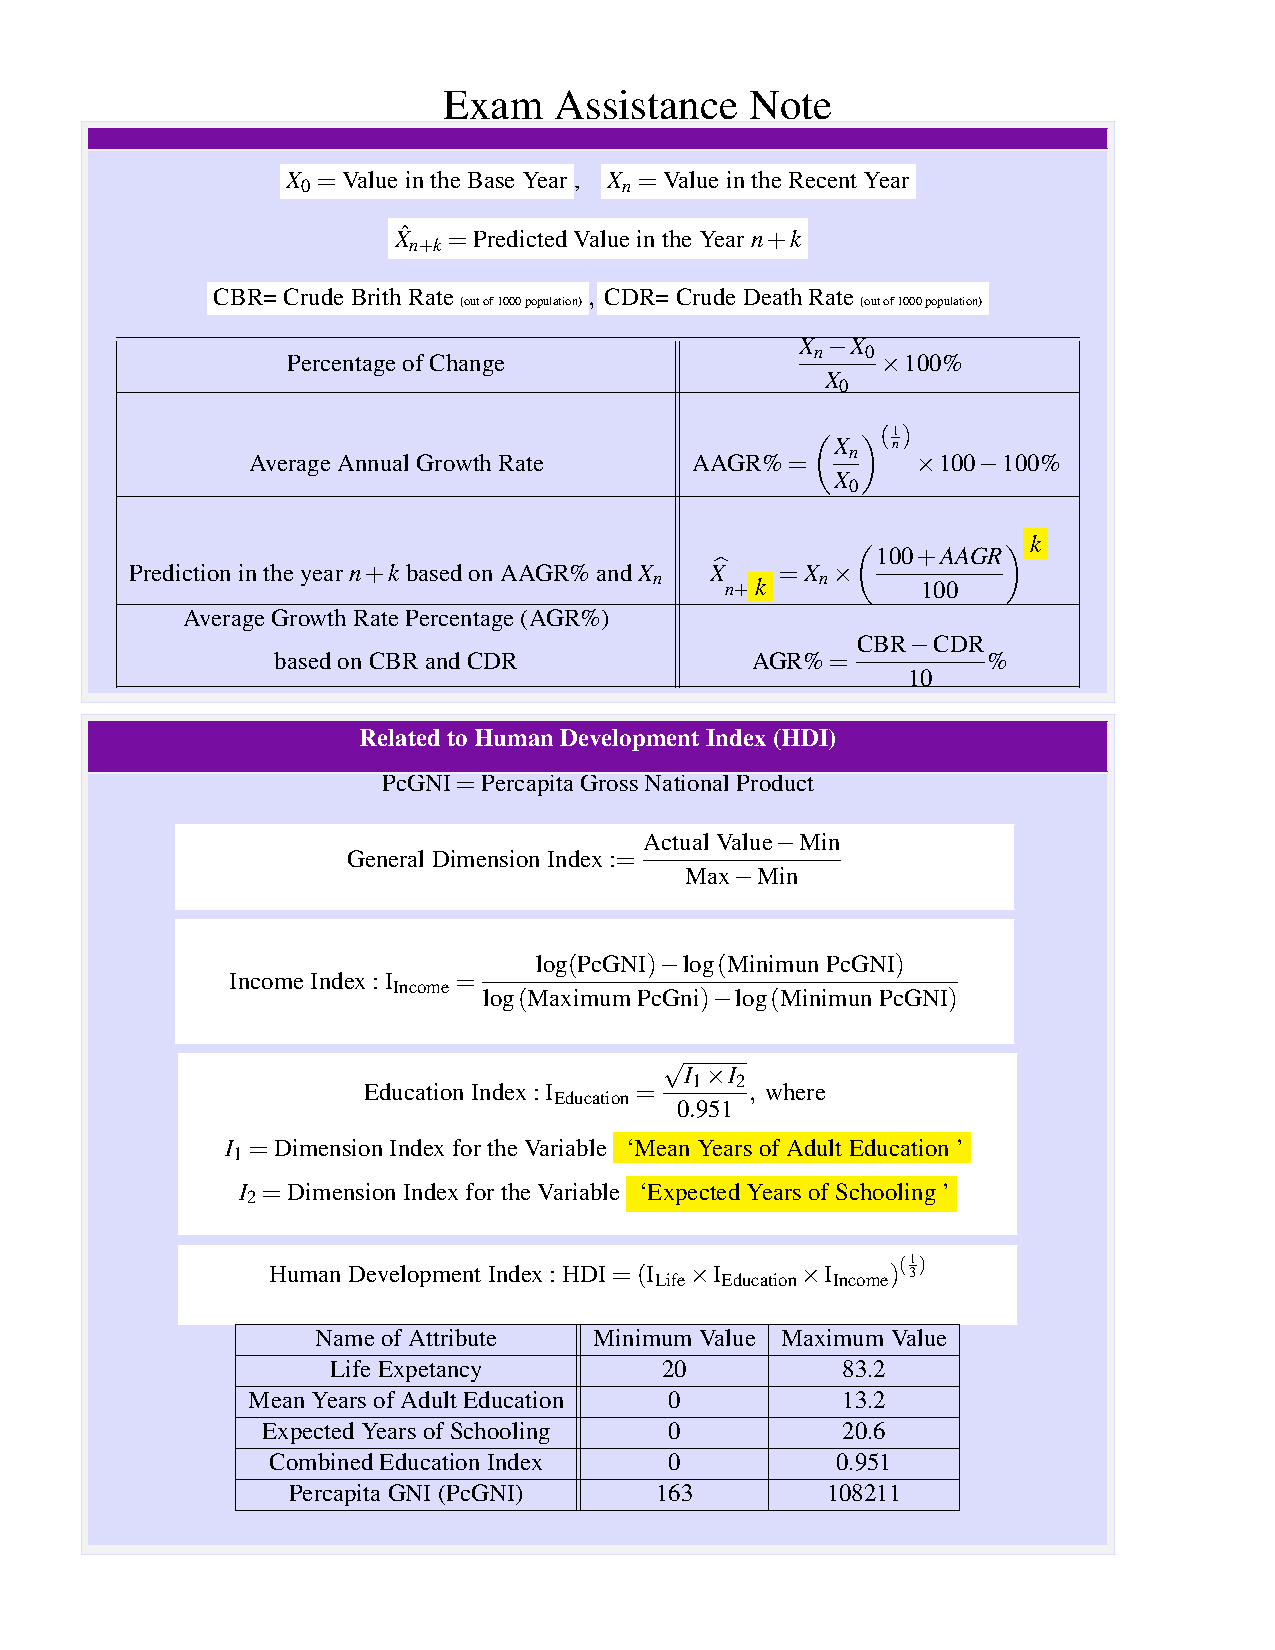
\includepdf[pages=-]{ExamAssistanceNote_STAt101.pdf}





\end{enumerate}
\end{document}